\chapter{LANDASAN TEORI}
% -------------------------------------------------------------------------------------------------------------------
% Konten:
% 1. Semantik web
% 2. Pemrosesan Bahasa Alami
% 3. Stemming ??? 
% 	a. algoritma stemming bahasa Indonesia ???
% 4. Ontologi
% 	a. Metode pembuatan ontologi
% 5. RDF
% 6. OWL Ontology
% 8. Ontologi Reasoning
% -------------------------------------------------------------------------------------------------------------------
Teknologi semantik web merupakan perluasan dari teknologi web yang telah ada saat ini atau lebih tepatnya adalah sebagai solusi dari kelemahan yang dimiliki oleh web saat ini. Seperti diketahui bahasa markup yang digunakan oleh web saat ini seperti HTML dan CSS hanya berfokus pada cara menampilkan dokumen saja tanpa memahami makna dari apa yang ditampilkannya. Akibatnya, komputer tidak dapat memproses data lebih jauh lagi, seperti misalnya melakukan penyimpulan (inferensi) serta bertukar informasi antar website tanpa harus melibatkan peran pengguna.

\citet{liyang_yu} menyebutkan bahwa tujuan dari semantik web yaitu untuk mendapatkan informasi sebanyak mungkin mengenai sesuatu yang ingin digali, sesuatu di sini dapat berupa orang, acara, produk dan lain sebagainya hanya dengan melakukan query terhadap sekumpulan data yang sudah tersedia dalam website. Saat ini,  tidak dapat mengetahui sebuah informasi yang terkandung dalam sebuah website hanya dengan melakukan query sederhana terhadap halaman web tersebut. Hal ini dikarenakan komputer tidak memahami informasi yang ditampilkannya.

Penggunaan website saat ini sudah cukup beragam mulai dari membaca berita, berinteraksi dengan pengguna lain melalui media sosial maupun pencarian data dengan menggunakan mesin pencari seperti Google, Yahoo, Bing dan lain sebagainya. Melakukan pencarian data saat ini merupakan salah satu aktifitas yang paling banyak dilakukan oleh pengguna internet, namun dengan semakin banyaknya jumlah sumber data yang tersebar di internet mengakibatkan timbulnya permasalah baru yaitu susahnya mendapatkan informasi yang relevan dengan yang kehendaki, sebagai contoh misalnya ingin mencari informasi mengenai program studi ilmu komputer Universitas Gadjah Mada dengan memasukkan kata kunci ``pascasarjana ilmu komputer UGM'' maka informasi yang akan dapatkan adalah tautan terhadap halaman-halaman yang mengandung kata-kata \emph{pascasarjana ilmu komputer ugm} yang jumlahnya dapat mencapai jutaan tautan. Hal ini tentunya akan menyebabkan proses untuk mendapatkan informasi yang sederhana seperti itu cukup memakan waktu karena selain  harus membuka tautan yang diberikan mesin pencari tadi juga harus membaca isi halaman tersebut untuk mengetahui apakah informasi yang disajikan sesuai dengan yang  kehendaki atau tidak. Untuk itulah semantik web hadir memberikan jawaban atas persoalan ini.

\section{Bahasa} % (fold)
\label{sec:section_name}
menurut \citet{chaer}, bahasa merupakan suatu lambang berupa bunyi, bersifat arbiter, digunakan oleh suatu masyarakat tutur untuk bekerja sama, berkomunikasi dan mengidentifikasi diri. \citet{dardjo} juga mengemukakan bahwa bahasa merupakan sistem simbol lisan yang arbiter yang dipakai oleh anggota suatu masyarakat bahasa untuk berkomunikasi dan berinteraksi antar sesamanya dengan berlandaskan pada budaya yang mereka miliki bersama.

Sebagai sebuah sistem, bahasa memiliki aturan, kaidah atau pola-pola tertentu, baik dalam tata bunyi, tata bentuk kata, maupun tata kalimat. Menurut \citet{dardjo}, bahasa disusun oleh tiga komponen, yaitu: sintaksis, fonologi, dan semantik. Komponen sintaksis adalah komponen yang menangani ihwal yang berkaitan dengan kata, frasa dan kalimat. Komponen fonologi adalah kompoenen yang menangani ihwal yang bekaitan dengan bunyi, sedangkan komponen semantik adalah komponen yang membahas ihwal makna.

\subsection{Kata}
Menurut \citet{chaer} melalui \citet{suryawan} bahwa kata merupakan perwujudan bahasa sehingga bahsa tidak akan ada jika kata tidak ada. Setiap kata mengandung konsep makna dan mempunyai peranan dalam pelaksanaan bahasa. \citet{alwi} mengelompokkan kata ke dalam empat kategori sintaksis utama yaitu: verba, nomina, adjektiva dan adverbia. Selain itu, ia juga memperkenalkan kelompok kata lain yang dinamakan kata tugas yang terdiri dari beberapa sub kelompok yang lebih kecil, yaiut: preposisi, konjungtor dan partikel.

\subsubsection{Verba (kata kerja)}
Kata-kata yang termasuk dalam kelompok kata kerja adalah kata-kata yang dapat diikuti loleh frasa \emph{dengan..} \citet{chaer}. Secara umum, verba berfungsi sebagai predikat atau inti predikat di dalam suatu kalimat \citep{alwi}.

Dilihat dari perilaku semantisnya, verba memiliki makna inheren yang terkandung di dalam verba itu sendiri. Verba dapat mengandung makna inheren \emph{perbuatan (aksi), proses} atau \emph{keadaan yang bukan sifat atau kuantitas} \citep{alwi}.

Secara sintaksi, verba dapat dikelompokkan ke dalam verba taktransitif dan verba transitif. Ketransitifan verba ditentukan oleh dua faktor yaitu: adanya nomina yang berfungsi sebagai ojek dalam kalimat aktif dan kemungkinan objek tersebut berfungsi sebagai subjek dalam kalimat pasif \citep{alwi}.
\begin{enumerate}
	\item \emph{Verba taktransitif}\\
	Adalah verba yang tidak diikuti oleh nomina yang berfungsi sebagai subjek dalam kalimat pasif. Verba taktransitif dibagi ke dalam tiga buah subkelompok yaitu: verba taktransitif tak berpelengkap, verba taktransitif berpelengkap wajib dan verba taktransitif berpelengkap manasuka.
	\item \emph{Verba transitif}\\
	Adalah verba yang memerlukan nomina sebagai objek dalam kalimat aktif dan objek tersebut dapat berfungsi sebagai subjek dalam kalimat pasif. Verba transitif dapat dibagi lagi ke dalam tiga kelompok, yaitu: verba ekatransitif, verba dwitransitif dan verba semitransitif.
\end{enumerate}

\subsubsection{Adjektiva (kata sifat)}
Adjektiva adalah kata yang memberikan keterangan yang lebih khusus tentang sesuatu yang  dinyatakan oleh nomina dalam suatu kalimat \citep{alwi}. Apabila ditinjau dari perilaku semantisnya, adjektiva dibagi menjadi dua kelompok yaitu:
\begin{enumerate}
	\item Adjektiva bertaraf, yaitu yang mengungkapkan suatu kualitas. Adjektiva bertaraf dibagi atas (1) adjektiva pemeri sifat, (2) adjektiva ukuran, (3) adjektiva warna, (4) adjektiva waktu, (5) ajdektiva jarak, (6) adjektiva sikap batin dan (7) adjektiva cerapan.
	\item Adjektiva tak bertaraf yang mengungkapkan keanggotaan dalam suatu golongan.
\end{enumerate}
Sedangkan dari segi sintaksisnya, adjektiva dapat berperilaku sebagi fungsi atribut, fungsi predikat, dan fungsi keterangan.

\subsubsection{Adverbia (kata keterangan)}
Adverbia adalah kata-kata yang digunakan untuk memberi penjelasan pada kalimat atau bagian kalimat lain, yang sifatnya tidak menerangkan keadaan atau sifat \citep{chaer}. Adverbia perlu dibedakan dalam tataran frasa dan dalam tataran klausa. Dalam tataran frasa, adverbia adalah kata yang menjelaskan verba, adjektiva dan adverbia lain. Sedangkan dalam tataran klausa, adverbia mewatasi atau menjelaskan fungsi-fungsi sintaksis \citep{alwi}.

\subsubsection{Nomina (kata beda)}
Kata benda adalah kata-kata yang dapat diikuti oleh frasa \emph{yang} ... atau \emph{yang sangat} ... \citep{chaer}. Dari segi bentuk morfologisnya, nomina dapat dibagi menjadi nomina dasar dan nomina turunan. Nomina dasar adalah nomina yang terdiri atas satu morfem sedangkan nomina turunan adalah nomina yang diturunkan melalui proses afiksasi, perulangan dan pemajmukan. Dari sisi semantisnya, kata benda mengacu pada manusia, binatang, benda dan konsep atau pengertian. \citet{alwi} mengungkapkan ciri-ciri nomina secara sintaksis adalah sebagai berikut:
\begin{enumerate}
	\item Dalam kalimat yang predikatnya berupa verba, nomina cenderung menduduki posisi sebagai subjek, objek atau pelengkap.
	
	\item Nomina tidak dapat diingkarkan dengan kata tidak.
	
	\item Nomina umumnya dapat diikuti dengan adjektiva, baik secara langsung maupun dengan diantarai oleh kata yang.
\end{enumerate}

\subsubsection{Pronomina}
Pronomina adalah kata yang digunakan untuk mengacu kepada nomina lain. \citet{alwi} melalui \citet{suryawan} mengungkapkan bahwa bahasa Indonesia mengenal tiga macam nomina yaitu:
\begin{enumerate}
	\item Pronomina persona\\
	Pronomina persona adalah pronomina yang digunakan untuk mengacu pada orang. Pronomina persona dapat mengacu pada diri sendiri (pronomina persona pertama), mengacu pada orang yang diajak bicara (pronomina persona kedua), atau mengacu pada orang yang dibicarakan (pronomina persona ketiga).

	\item Pronomina penunjuk\\
	Bahasa indonesia memiliki tiga macam pronomina penunjuk, yaitu: pronomina penunjuk umum, pronomina penunjuk tempat dan pronomina penunjuk ihwal. Pronomina penunjuk umum dapat mandiri sepenuhnya sebagai nomina. Sebagai nomina, pronomina penunjuk umum dapat berfungsi sebagai subjek atau objek kalimat, dan bahkan dapat pula berfungsi sebagai predikat dalam kalimat yang berpredikat nomina.

	\item Pronomina penanya\\
	Pronomina penanya adalah pronomina yang dipakai sebagai pemarkah pertanyaan. Dari segi maknanya, yang ditanyakan dapat mengenai orang, barang, atau pilihan. Ditinjau dari segi bentuknya, kata penanya didasari oleh dua bentuk yaitu: \emph{apa} dan \emph{mana}. Unsur dasar tersebut dapat dikembangkan menjadi bentuk lain seperti apa, siapa, mengapa, kenapa, kapan, dimana, kemana dan bagaimana.
\end{enumerate}

\subsubsection{Numeralia (kata bilangan)}
Numeralia adalah kata yang digunakan untuk menghitung banyaknya maujud (orang, binatang atau barang) dan konsep. Bahasa Indonesia mengenal dua macam numeralia, yaitu: numeralia pokok (numeralia kardinal) dan numeralia tingkat (numeralia ordinal) \citep{alwi}

\subsubsection{Preposisi (kata depan)}
Preposisi dalam bahasa Indonesia berfungsi sebagai penanda hubungan tempat, peruntukan, sebab, kesertaan atau cara, pelaku, waktu, ihwal (persitiwa) dan milik. Dilihat dari perilaku sintaksisnya, preposisi berada di depan nomina, adjektiva atau adverbia, sedangkan jikal dilihat dari bentuk sintaksisnya, preposisi dapat dibagi menjadi preposisi tunggal dan preposisi majemuk \citep{alwi}

\subsubsection{Konjungtor (kata sambung)}
Konjungtor adalah kata tugas yang menghubungkan dua satuan bahasa yang sederajat: kata dengan kata, frasa dengan frasa, atau klausa dengan kalusa. Dilihat dari perilaku sintaksisnya dalam kalimat, konjungtor dapat dibagi menjadi empat kelompok, yaitu: konjungtor koordinatif, konjungtor subordinatif, konjungtor korelatif dan konjungtor antar kalimat \citep{alwi}

\subsubsection{Interjeksi (kata seru)}
Interjeksi adalah kata tugas yang digunakan untuk mengungkapkan rasa hati pembicara. Interjeksi umumnya ditempatkan di awal kalimat dan pada penulisannya diikuti oleh tanda koma. Secara struktural, interjeksi tidak bertalian dengan unsur kalimat yang lain \citep{alwi}.

\subsubsection{Artikula}
Artikula adalah kata tugas yang membatasi makna nomina. Bahasa Indonesia membagi artikula ke dalam tiga kelompok, yaitu: artikula yang bersifat gelar, artikula yang mengacu ke makna kelompok, dan artikula yang menominalkan \citep{alwi}.

\subsubsection{Partikel Penegas}
Partikel penegas adalah morfem-morfem yang digunakan untuk menegaskan \citep{chaer}. Partikel penegas meliputi kata yang tidak tertakluk pada perubahan bentuk dan hanya berfungsi untuk menampilkan unsur yang diiringinya. Bahasa Indonesia memiliki empat partikel pengas, yaitu: \emph{-lah, -kah, -tah} dan \emph{-pun} \citep{alwi}.

\subsection{Frasa}
Frasa adalah gabungan dua buah kata atau lebih yang merupakan satu kesatuan. Tujuan dari penggabungan dua kata atau lebih menjadi satu kesatuan adalah untuk menampung konsep makna yang lebih khas atau lebih tertentu yang tidak dapat diwujudkan dengan sebuah kata saja \citep{chaer}. Secara sintaksis, frasa dapat dikelompokkan ke dalam frasa verbal, frasa nominal, frasa pronominal, frasa numeralia dan frasa preposisional. 

\subsubsection{Frasa Verbal}
Frasa verbal adalah satuan bahasa bukan klausa yang terbentuk dari dua kata atau lebih dengan verba sebagai intinya \citep{alwi}. Suatu bahasa yang dapat mendampingi verba dalam frasa verbal dapat berupa frasa nominal, klausa pemerlengkap dan atau frasa preposisional \citep{lapoliwa}.

\subsubsection{Frasa Nominal}
Frasa nominal dapat dibentuk dari nomina yang didahului oleh frasa numeral dan atau diikuti oleh frasa nominal, frasa verbal, frasa preposisional, klausa dan atau penentu. Frasa nominal juga dapat dibentuk dari klausa (sebagai pemerlengkapan) yang dapat didahului oleh nomina \citep{lapoliwa}
Menurut \citet{alwi}, frasa nominal dapat dibentuk dari nomina dengan memperluas nomina tersebut ke kiri dan atau ke kanan. Perluasan ke kiri dilakukan dengan meletakkan frasa numeralia di depan nomina. Perluasan ke kanan dapat memiliki bebrapa macam bentuk dengan mengikuti kaidah sebagai berikut:
\begin{enumerate}
	\item Suatu inti dapat diikuti oleh suatu nomina lain atau lebih. Rangkaian tersebut dapat ditutup oleh pronomina persona dan pronomina penunjuk \emph{ini} atau \emph{itu}.
	
	\item Suatu inti dapat diikuti oleh adjektiva, pronomina atau frasa pemilikan, dan kemudian ditutup dengan pronomina penunjut \emph{ini} atau \emph{itu}.
	
	\item Jika suatu nomina diikuti oleh adjektiva dan tidak terdapat pewatas lain yang mengikutinya, kata \emph{yang} dapat disisipkan di antara nomina dan adjektiva. Akan tetapi kata \emph{yang} dan adjektiva harus dipindah ke belakang jika di dalam frasa tersebut terdapat pronomina.

	\item Suatu inti dapat diikuti verba tertentu yang pada hakikatnya dapat dipisahkan oleh kata \emph{yang}, \emph{untuk}, atau unsur tertentu.

	\item Suatu inti dapat diperluas dengan aposisi, yaitu frasa nominal yang mempunyai acuan yang sama dengan nomina yang diterangkannya.

	\item Suatu inti dapat diperluas dengan pewatas belakang, yakni kalusa yang dimulai dengan kata \emph{yang}.

	\item Suatu inti dapat diperluas oleh frasa preposisional. Frasa preposisional yang menjadi pewatas nomina tersebut merupakan bagian dari frasa nominal sehingga tidak dapat dipindahkan ke tempat lain. 
\end{enumerate}

\subsubsection{Frasa Pronominal}
Pronomina dapat diperluas menjadi frasa pronominal. Menurut \citet{alwi}, perluasan pronominal menjadi frasa pronominal dapat dilakukan dengan menambahkan numeralia kolektif, menambahkan kata penunjuk, menambahkan kata \emph{sendiri}, menambahkan klausa yang diawali oleh kata \emph{yang}, atau menambahkan frasa nominal yang memiliki funsi apositif.

\subsubsection{Frasa Numeralia}
Menurut \citet{alwi}, numeralia dapat diperlias menjadi frasa numeralia. Frasa numeralia dapat dibentuk dengan menambahkan kata penggolong di belakang numeralia.

\subsubsection{Frasa Preposisional}
Frasa preposisional dibentuk dari preposisidan frasa nominal. Meskipun frasa preposisional mempunyai makna yang beragam, Struktur frasa preposisional relatif seragam \citep{lapoliwa}.

\subsection{Kalimat}
Kalimat adalah satuan bahasa terkecil, dalam wujud lisan atau tulisan, yang mengungkapkan pikiran yang utuh. Dalam wujud lisan, kalimat diucapkan dengan suara naik turun dan keras lembut, disela jeda, dan diakhiri dengan intonasi akhir yang diikuti dengan kesenyapan. Dalam wujud tulisan berhuruf Latin, kalimat dimulai dengan huruf kapital dan diakhiri dengan tanda titik (.), tanda tanya (?), atau tanda seru (!). Sementara itu, di dalamnya dapat disertakan berbagai tanda baca seperti koma (,), titik dua (:), tanda pisah (-) dan spasi \citep{alwi}.

Menurut \citet{alwi}, kalimat merupakan konstruksi sintaksi terbesar yang terdiri dari dua kata atau lebih. Penggabungan dua kata atau lebih dalam satu kalimat menuntut adanya keserasian diantara unsur-unsur tersebut, baik dari segi makna maupun dari segi bentuk.

Kalimat dapat dikelompokkan berdasarkan jumlah kalusa yang menyusun kalimat. Klausa merupakan satuan sintaksis yang terdiri dari dua kata atau lebih yang mengandung unsur predikasi. Menurut \citet{alwi}, berdasarkan jumlah klausanya, kalimat dapat dibedakan menjadi:
\begin{enumerate}
	\item kalimat tunggal\\
	Kalimat tunggal adalah kalimat yang terdiri atas satu klausa. sehingga konstituen untuk unsur subjek dan predikat hanya ada satu atau merupakan datu kesatuan. Kalimat tunggal dapat mengandung unsur manasuka seperti keterangan tempat, waktu dan alat.

	\citet{alwi} melalui \citet{suryawan} membagi kalimat tunggal berdasarkan kategori predikatnya ke dalam kalimat  berpredikat verbal, kalimat berpredikat adjektival, kalimat berpredikat nominal (termasuk pronominal), kalimat berpredikat numeral dan kalimat berpredikat preposisional.

	\item Kalimat majemuk\\
	kalimat majemuk disusun oleh lebih dari satu klausa. Klausa-klausa yang terdapat di dalam kalimat majemuk bertingkat dapat dihubungkan dengan dua cara, yaitu: koordinasi dan subordinasi.

	Koordinasi adalah menghubungkan dua klausa atau lebih yang memiliki kedudukan konstituen sama. Kalimat majemuk yang dibentuk dengan menggunakan koordinasi disebut dengan \emph{kalimat majemuk setara}.

	Subordinasi adalah menguhubungkan dua klausa atau lebih yang kedudukan konstituennya tidak sama. Hubungan yang dibangun dengan menggunakan subordinasi dapat bersifat melengkapi (komplementatif) atau bersifat mewatasi atau menerangkat (atributif). Klimat majemuk yang dibentuk dengan menggunakan subordinasi disebut dengan \emph{kalimat majemuk bertingkat}.
\end{enumerate}

Kalimat dapat dikelompokkan berdasarkan bentuk atau kategori sintaksis dari kalimat. Berdasarkan bentuk atau kategori sintakasisnya, kalimat dapat dibagi ke dalam empat kelompok, yaitu:
\begin{enumerate}
	\item Kalimat berita (kalimat deklaratif)\\
	Kalimat deklaratif umumnya digunakan untuk menyampaikan pernyataan sehingga isinya merupakan berita bagi pendengar atau pembacanya. Kalimat deklaratif tidak memiliki markah khusus, sehingga kalimat berita dapat berupa bentuk apa saja. Dalam bentuk tulisan, kalimat deklaratif diakhiri dengan tanda titik. Dalam bentuk lisan, kalimat berita diakhiri dengan nada turun.

	\item Kalimat perintah (kalimat imperatif)\\
	\citet{dardjo_et_al} mendefiniskan kalimat imperatif sebagai kalimat yang maknanya meberikan perintah untuk melakukan sesuatu. Dalam bentuk tulisan, kalimat imperatif diakhiri dengan menggunakan tanda seru (!). Dalam bentuk lisan, kalimat imperatif ditandai dengan nada yang semakin tinggi.

	\item Kalimat tanya (kalimat interogatif)\\
	\citet{dardjo_et_al} mendefinisikan kalimat interogatif sebagai kalimat yang isinya menanyakan sesuatu atau seseorang. Kalimat interogatif secara formal ditandai dengan kehadiran kata tanya seperti \emph{apa}, \emph{siapa}, \emph{berapa}, \emph{kapan} dan \emph{bagaimana}, dengan atau tanpa partikel penegas \emph{-kah}. Pada bahasa tulis, kalimat interogatif ditandai dengan tanda tanya (?). Pada bahasa lisan, kalimat tanya ditandai dengan suara naik jika kalimat memiliki kata tanya dan suara turun jika kalimat tidak memiliki kat tanya \citep{alwi}.

	Kalimat interogatif umumnya dibentuk dari kalimat deklaratif. Berikut adalah kaidah pembentukan kalimat tanya dari kalimat deklaratif menurut \citet{alwi}:

	\begin{enumerate}
		\item Kalimat tanya dapat dibentuk dari kalimat deklaratif dengan menambahkan pronomina penanya \emph{apa} pada kalimat tersebut. Partikel \emph{-kah} dapat ditambahkan pada pronomina penanya untuk mempertegas pertanyaan tersebut.

		\item Kalimat tanya dapat dibentuk dengan cara mengubah urutan kata dari kalimat deklaratif. Kaidah yang perlu diperhatikan dalam pembentukan kalimat tanya adalah sebagai berikut:
		\begin{enumerate}
			\item Jika dalam kalimat deklaratif terdapat kata seperti \emph{dapt, bisa, harus, sudah} dan \emph{mau}, maka kata tersebut dipindahkan ke awal kalimat dan ditambahkan partikel \emph{-kah}.

			\item Jika predikat dari kalimat berupa nomina atau adjektiva, urutan subjek dan predikatnya dapat dibalik kemudian partikel \emph{-kah} ditambahkan pada frasa yang telah dipindahkan ke awal kalimat.

			\item Jika predikat kalimat berupa verba taktrasitif, ekatransitif atau semitransitif, maka verba beserta objek atau pelengkapnya dapat dipindahkan ke awal kalimat dan kemudian ditambahkan partikel \emph{-kah}.
		\end{enumerate}

		\item Kalimat tanya dapat dibentuk dengan menempatkan kata \emph{bukan/bukankah, (apa/apakah) belum} atau \emph{tidak}.

		\item Kalimat tanya dapat dibentuk dengan mempertahankan urutan kata seperti dalam kalimat deklaratif, tetapi pengucapannya menggunakan intonasi yang naik.

		\item Kalimat tanya dapat dibentuk dengan menggunakan pronomina interogatif seperti \emph{apa, siapa, mengapa, kenapa, kapan, (Ke)berapa, dimana, kemana, dari mana, bagaimana} dan \emph{bilamana}.
	\end{enumerate}

	\item Kalimat seru (kalimat eksklamatif)\\
	Kalimat seru atau kalimat eksklamatif juga dikenal dengan sebutan kalimat interjeksi. Kalimat seru dapat digunakan untuk menyatakan perasaan kagum atau heran \citep{alwi}. \citet{chaer} menyatakan bahwa kalimat seru juga dapat digunakan untuk menyatakan emosi atau perasaan batin yang biasanya terjadi secara tiba-tiba.
\end{enumerate}

Kalimat dapat dikelompokkan berdasarkan kelengkapan unsur-unsur yang menyusun kalimat. Berdasakan kelengkapan unsurnya, kalimat dapat dikelompokkan ke dalam kalimat lengkap (kalimat major) dan kalimat tak lengkap (kalimat minor). Kalimat lengkap adalah kalimat yang memiliki unsur subjek dan predikat. Kalimat tak lengkap adalah kalimat yang tidak memiliki unsur subjek dan/ atau predikat. Kalimat tak lengkap umumnya muncul di dalam wacana dimana unsur yang tidak muncul tersebut sudah diketahui atau disebutkan sebelumnya \citep{alwi}.
% section section_name (end)
\section{Pengolahan Bahasa Alami}
Pemrosesan bahasa alami atau \emph{Natural Language Processing (NLP)} merupakan salah satu bidang yang tidak dapat dipisahkan dari sebuah sistem \emph{question answering}. Kata kunci pencarian dalam sistem \emph{question answering} umumnya berupa bahasa alami sesuai dengan bahasa yang dipahami oleh pengguna, untuk itu pengolahan bahasa alami bertindak sebagai pemroses awal yang akan mengubah kalimat tanya yang diajukan oleh pengguna menjadi pohon urai \emph{(parse tree)} sehingga dapat diphamai oleh komputer.

Tujuan dari pengolahan bahasa alami adalah untuk membuat model komputasi dari bahasa, sehingga memungkinkan manusia berinteraksi dengan komputer dengan menggunakan bahasa alami.

\citet*{kao_potet} menjelaskan bahwa pengolahan bahasa alami (NLP) adalah usaha untuk mendapatkan representasi makna dari \emph{free text}.

Pengolahan bahasa alami memiliki beberapa tingkat pengolahan yaitu:
\begin{enumerate}
	\item Fonetik dan fonologi \\
		Tingkat ini berhubungan dengan suara yang menghasilkan kata yang dapat dikenali. Bidang ini penting untuk sebuah sistem yang berfokus pada sistem pengenalan suara \emph{(speech recognation).}
	\item Morfologi \\
		Pengetahuan tentang kata dan bentuknya dimafaatkan untuk membedakan satu kata dengan lainnya. Pada tingkat ini juga dapat dipisahkan antara kata dan elemen lain seperti tanda baca.
	\item Sintaksis \\
		Pemahaman tentang urutan kata dalam pembentukan kalimat dan hubungan antar kata tersebut dalam proses perubahan bentuk dari kalimat menjadi bentuk yang sistematis. Meliputi proses pengaturan tata letak suatu kata dalam kalimat akan membentuk kalimat yang dapat dikenali. Selain itu pula dikenali bagian-bagian kalimat dalam suatu kalimat yang lebih besar. Sebagai contoh kalimat S dibentuk dari noun phrase (NP) dan verb phrase (VP)
		\begin{lstlisting}[language=Python,xleftmargin=0pt]
			S -> NP,VP
			dan berikutnya:
			NP -> DET,N
			VP -> V,NP
			NP -> N
		\end{lstlisting}
	\item Semantik\\
		Pemetaan bentuk sturktur sintaksis dengan memanfaatkan tiap kata ke dalam bentuk yang lebih mendasar dan tidak tergantung struktur kalimat. Semantik mempelajari arti suatu kata dan bagaimana dari arti kata - arti kita tersebut membentuk suatu arti dari kalimat yang utuh. Dalam tingkatan ini belum tercakup konteks dari kalimat tersebut.
	\item Pragmatik\\
		Penegtahuan pada tingkatan ini berkaitan dengan masing-masing konteks yang berbeda tergantung pada situasi dan tujuan pembuatan sistem.
	\item Discourse knowledge
		Tingkatan ini melakukan pengenalan apakah suatu kalimat yang sudah dibaca dan dikenali sebelumnya akan mempengaruhi arti dari kalimat selanjutnya. Informasi ini penting diketahui untuk melakukan pengolahan arti terhadap kata ganti orang dan untuk mengartikan aspek sementara dari informasi.
	\item World knowledge\\
		Mencakup arti sebuah kata secara umum dan apakah ada arti secara khusus bagi suatu kata dalam suatu percakapan dengan konteks tertentu.
\end{enumerate}

Definisi ini tidaklah bersifat kaku, dan untuk setiap bentuk bahasa alami yang ada biasanya ada pendefinisian lagi yang lebih spesifik sesuai dengan katater bahasa tertentu. Pada beberapa masalah mungkin hanya mengambil beberapa dari pendekatan tersebut bahkan mungkin ada yang melakukan tembahan proses sesuai dengan karakter dari bahasa yang digunakan dan sistem yang dibentuk.

Selain yang sudah disebutkan diatas, masih ada lagi satu masalah yang cukup menantang dalam bidang pengolahan bahasa alami yaitu masalah ambiguitas atau makna ganda dari satu buah kata atau kalimat. Dari satu masukan yang sama dapat dapat menjadi beberapa arti yang berbeda dan masing-masing dapat bernilai benar tergantung pada keperluan pemakai. Hal ini dapat terjadi pada hampir semua tingakatan pendekatan di atas.
\section{Gramatika}
Grammar suatu bahasa dapat dilihat sebagai suatu aturan yang menentukan apakah suatu kumpulan kata dapat diterima sebagai kalimat oleh bahasa tersebut. Sebuah bahasa L dapat dijelaskan sebagai se dari \emph{string}, dimana \emph{string} dibentuk dari bagian terkecil yang disebut dengan \emph{symbol}.

Sebuah \emph{grammar} G dinyatakan dalam persamaan 
\section{Parsing}
Parsing merupakan proses menganalisa sekumpulan kata berdasarkan grammar tertentu
% \section{\emph{Resource Description Framework}}
\emph{Resource Description Framewok (RDF)} merupakan dasar pembentuk basis pengetahuan dalam semantik web, diajukan oleh W3C sebagai standar pada tahun 1999. RDF terdiri dari subjek, predikat dan objek yang kemudian dikenal dengan naman \emph{statement}. Subjek dapat berupa URI (Uniform Resource Identifier) yang berfungsi sebagai penanda atau \emph{identifier}, tidak menuntup kemungkinan sebuah subjek juga dapat berupa URL \emph{(Uniform Resource Locator)} yang merupakan bentuk khusus dari URI.  Predikat berupa URI yang menjelaskan hubungan antara subjek dengan objeknya sedangkan objek dapat berupa URI ataupun \emph{literal}. Sebuah pernyataan dalam RDF disebut dengan istilah \emph{triple}. secara grafis, bentuk \emph{statement} RDF dapat dilihat pada gambar \ref{fig:rdf_statement}.

\begin{figure}[!]
	\centering
	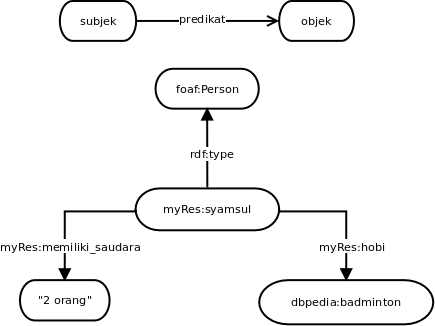
\includegraphics[trim = 29mm 141mm 40mm 0mm, clip, scale=0.6]{gambar}
	\caption{Struktur \emph{statement} RDF}
	\label{fig:rdf_statement}
\end{figure}

Sebagai contoh misalnya pernyataan ``Syamsul hobi badminton'', ``Syamsul memiliki saudara 2 orang'', pernyataan-pernyataan tersebut dapat dibentuk menjadi sebuah \emph{triple}. Pada pernyataan pertama, \emph{Syamsul} adalah merupakan subjek sedangkan \emph{hobi} merupakan sebuah predikat dan \emph{badminton} merupakan sebuah objek, sedangkan pada pernyataan kedua yang menjadi subjek adalah \emph{Syamsul} sedangkan predikat adalah \emph{memmiliki saudara} dan \emph{2 orang} merupakan objek. Jika objek pada pernyataan pertama di atas memerlukan penjelasan lebih lanjut, misalnya mengenai apa itu badminton, maka objek tersebut dapat berupa \emph{resource} dimana \emph{resource} tersebut membentuk triple-triple seperti terlihat pada gambar \ref{fig:rdf_multi_statement}. Pada pernyataan kedua, hanya dimungkinkan berupa literal karena tidak memerlukan penjelasan lebih lanjut mengenai objek itu sendiri.

Agar dapat di proses oleh komputer maka RDF triple harus dituliskan dalam bahasa atau sintak yang dapat dimengerti oleh komputer. Hingga saat ini bentuk penulisan RDF yang direkomendasikan oleh W3C adalah dalam bentuk XML dengan menggunakan namespace yang khusus RDF. Contoh statement di atas dapat kita serialisasi menjadi RDF sebagai berikut:
\lstinputlisting[firstline=1, lastline=7]{./parts/codeblock.xml}
\begin{figure}[!]
	\centering
	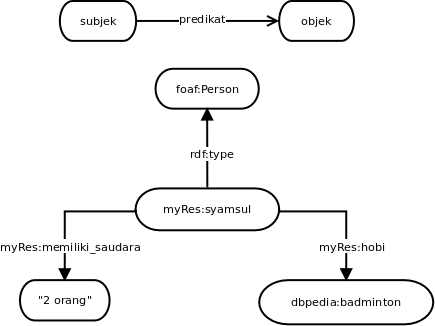
\includegraphics[trim = 0mm 0mm 0mm 93mm, clip, scale=0.55]{gambar}
	\caption{RDF dengan multi-statement}
	\label{fig:rdf_multi_statement}
\end{figure}
Selain XML/RDF, RDF juga dapat dituliskan dengan menggunakan Turtle sintaks sebagai berikut:
\lstinputlisting[firstline=9, lastline=11]{./parts/codeblock.xml}

Sintaks turtle lebih mudah dipahami oleh manusia, sehingga lebih mudah dibentuk. Meskipun sintak ini masih belum menjadi rekomendasi W3C namun besar kemungkinan kedepan juga akan menjadi rekomendasi karena sudah memiliki draft yang dapat dilihat di http://www.w3.org/TR/turtle/.
% \section{\emph{RDF Schema}}
Dalam kasus yang lebih kompleks, RDF tidak cukup kuat untuk menjelaskan semantik dari sebuah subjek yang sedang dijelaskan. Jika kita kembali pada contoh di atas, apabila kita ingin lebih jauh menjelaskan mengenai misalnya apa/siapa Syamsul Muttaqin, RDF tidak dapat menjelaskan hal ini \citep*{antoniou}. Untuk mengatasi hal ini, maka di diperkenalkan RDF Schema (RDFS).

\begin{figure}[h]
	\centering
	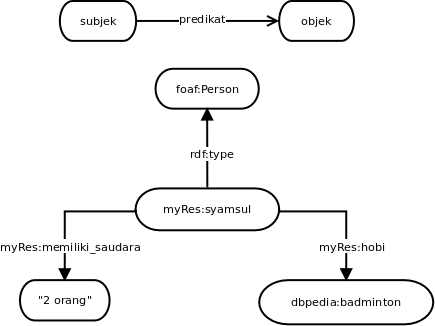
\includegraphics[trim = 0mm 0mm 0mm 32mm, clip, scale=0.55]{gambar}
	\caption{RDFS-statement}
	\label{fig:rdfs_statement}
\end{figure}

Sesuai dengan namanya, RDF Schema memberikan penjelasan lebih jauh mengenai objek yang sedang dibicarakan. Untuk itu RDFS diperkaya dengan beberapa penambahan namespace seperti rdfs:Class yang digunakan untuk menjelaskan tipe dari sebuah objek, rdfs:subClassOf yang merupakan turunan dari kelas, rdfs:domain, rdfs:range, serta beberapa penambahan lainnya. Gambar \ref{fig:rdfs_statement} menunjukkan RDFS statement, dimana \emph{foaf:Person} adalah kelas dan \emph{myRef:syamsul} merupakan \emph{instance} dari kelas \emph{Person}.
\section{Ontologi}
Ontologi memiliki peranan penting dalam semantik web. Terdapat berbagai definisi ontologi dalam bidanng semantik web, menurut T.R Gruber melalui \citet*{antoniou}, ontologi adalah \emph{spesifikasi formal dari sebuh konseptualisasi}, sedangkan W3C melalui \citet{liyang_yu} mendefinisikan ontologi sebagai \emph{definisi formal dari sekumpulan term yang digunakan untuk mendeskripsikan dan merepeserentasikan sebuah domain tertentu.}

Ontologi berfungsi sebagai media untuk berbagi pengetahuan dan pemahaman terhadap sesuatu antara domain atau berbagi terminologi yang berbeda namun memliki makna yang sama, misalnya \emph{ZIP Code} sama dengan Kode Wilayah di Indonesia, dengan demikian apabila seseorang mencari dengan menggunakan kata kunci kode wilayah untuk suatu daerah di Amerika misalnya, maka komputer akan dapat memahami bahwa yang dimaksud adalah ZIP Code, demikian juga sebaliknya.

\subsection{Metode pengembangan ontologi}
\citet{fernandez_lopez} dalam \citet*{fonou_huisman} menyebutkan berbagai macam metode yang dapat digunakan untuk pengembangan ontologi, namun demikian \citet{noy_mcguinness} mengungkapkan bahwa tidak ada satu metode yang pasti dalam mengembangkan ontologi. Ia juga mengungkapkan sesungguhnya proses pembuatan ontologi adalah sebuah proses iteratif yang tidak dapat dikerjakan hanya dalam satu tahapan saja, bahkan sangat mungkin pengembangan ontologi terus berlanjut meskipun ontologi sudah digunakan. 

Pemilihan metode pengembangan tergantung pada masing-masing pengembang ontologi, seperti misalnya \citet*{fonou_huisman} memilih menggunakan metode yang dikembangkan oleh \citet*{uschold_king} dengan alasan bahwa metode ini lebih mudah dipahami bagi para pengembang ontologi pemula.

\citet{noy_mcguinness} menawarkan salah satu metode pengembangan ontologi yang didasakan pada pengalaman mereka dalam mengembangkan ontologi. Metode ini paling banyak digunakan dalam pengembangan ontologi. Secara umum tahapan yang harus dilalui dalam pengembangan ontologi adalah sebagai berikut:
\begin{enumerate}
	\item Tentukan domain dan ruang lingkup \emph{scope} dari ontologi\\
	Untuk membantu dalam menentukan domain dan ruang lingkup dari ontologi yang akan dibangun, seorang ahli ontologi \emph{ontology engineer} harus dapat menjawab pertanyaan:
	\begin{enumerate}
		\item Domain apa yang ingin ditangani oleh ontologi ini ?
		\item Akan digunakan untuk apa ontologi ini ?
		\item Pertanyaan seperti apa yang harus dapat dijawab oleh ontologi ini ?
	\end{enumerate}
	Jawaban atas pertanyaan-pertanyaan tersebut mungkin saja dapat berubah selama proses pengembangan ontologi berlangsung, namun setidaknya dapat membantu untuk memastikan ontologi yang akan dibangun tidak keluar dari rung lingkup yang sudah ditetapkan.
	\item Gunakan ontologi yang sudah ada\\
	Sebelum mulai mengembangkan ontologi, ada baiknya untuk mencari apakah ontologi yang akan dibuat sudah pernah dibuat atau belum. Jika sudah ada, apabila memenuhi kriteria yang diinginkan maka sebaiknya menggunakan ontologi tersebut.
	\item Tentukan semua \emph{term} penting dalam ontologi\\
	Tentukan semua \emph{term} baik berupa kelas, objek properti maupun \emph{datatype property} dari ontologi domain yang akan ditangani.
	\item Buat semua kelas dan strukturnya\\
	Pada tahapan ini, kelas-kelas yang akan di representasikan dalam domain dibuat terlebih dahulu, kemudian diikuti dengan membuat relasi antar kelas-kelas tersebut. Relasi disini termasuk struktur sub dan super kelas. Untuk menentukan struktur relasi dapat menggunakan metode \emph{top-down, bottom-up} atau kombinasi keduanya.
	\item Buat properti kelas - \emph{slot}\\
	Setelah proses pembuatan kelas selesai, selanjutnya buat juga properti yang akan digunakan pada kelas-kelas yang sudah dibuat.
	\item Tentukan \emph{facet} dari \emph{slot}\\
	\emph{Facet} menjelaskan mengenai tipe nilai dari kelas, nilai yang diperbolehkan, jumlah yang diperbolehkan \emph{(cardinality)}.
	\item Buat anggota dari kelas \emph{(instance)}\\
	Langkah terakhir adalah membuat anggota atau \emph{instance} dari masing-masing kelas.
\end{enumerate}
\section{OWL Ontologi}
OWL \emph{(Web Ontology Language)} dijadikan sebagai rekomendasi formal oleh W3C pada 10 februari 2004 \citep{liyang_yu}. OWL dirancang untuk kompatibel dengan sintak XML. OWL merupakan pengembangan RDF dan RDFS yang menjadi rekomendasi W3C sebelumnya, oleh karena itu secara sintaksis OWL kompatibel dengan sintak RDF dan RDF Schema.

Ide awal dari pengembangan OWL berdasarkan fakta bahwa RDF Schema belum cukup kuat dalam mereperesentasikan semantik dari sebuah \emph{statement} sehingga diperlukan definisi lebih lanjut. Definisi inilah yang kemudian diperkenalkan dalam OWL. \citet*{antoniou} menjelaskan beberapa model semantik yang tidak dapat dituangkan dalam RDF Schema diantaranya :
\begin{enumerate}
	\item Cakupan \emph{(scope)} dari sebuah properti. Sebagai contoh misalnya properti atau predikat \textit{memakan}, RDFS tidak dapat membatasi range cakupan properti ini hanya untuk kelas tertentu, misalnya kita tidak dapat menyebutkan ``Sapi hanya memakan rumput'', sementara sapi sendiri merupakan \emph{instance} dari kelas binatang, dimana kelas ini tidak hanya berisi sapi saja, namun juga dapat berisi kucing, sementara kucing tidak memakan rumput.
	\item \emph{Disjoint} antar kelas. RDFS hanya menjelaskan mengenai hirarki kelas--sub-kelas, ia tidak dapat membedakan apakah dua atau lebih kelas yang berbeda atau tidak. Sebagai contoh, misalnya kita ingin mendefinisikan kelas mobil dan motor adalah dua kelas yang berbeda, yang artinya apabila \emph{x} adalah \emph{instance} dari kelas motor, maka \emph{x} tidak mungkin menjadi \emph{instance} dari kelas mobil. RDFS tidak memiliki properti untuk menjelaskan hal ini, ia hanya dapat menjelaskan bahwa kedua kelas tersebut adalah merupakan sub-kelas dari kelas induk yaitu kendaraan.
	\item Kelas kombinasi. RDFS tidak dapat mendefinisikan sebuah kelas baru yang merupakan gabungan (union) dari dua atau lebih kelas lain. RDFS juga tidak dapat mendefinisikan bentuk kombinasi lain seperti irisan atau \emph{intersection} ataupun komplemen dari dua buah kelas yang berbeda. Misalnya kelas Kendaraan adalah gabungan dari kelas Mobil dan Motor.
\end{enumerate}
Sebuah dokumen OWL terdiri dari elemen header, elemen kelas, elemen properti, elemen restriksi properti, elemen properti khusus, serta elemen kombinasi boolean. 

\subsection{Elemen \emph{header}}
Sesuai dengan standar aturan XML dimana sebuah file terdiri dari sebuah elemen \emph{root}, elemen \emph{root} dari OWL adalah rdf:RDF dimana pada elemen \emph{root} ini dideklarasikan pula beberapa \emph{namespace} yang menjadi standar seperti terlihat pada gambar \ref{fig:deklarasi_header_owl} berikut:
\begin{figure}[ht]
	\centering
	\lstinputlisting[firstline=13, lastline=16, xleftmargin=0pt]{./parts/codeblock.xml}
	\caption{Contoh deklarasi \emph{header} OWL}
	\label{fig:deklarasi_header_owl}
\end{figure}

Header terdapat diantara elemen \texttt{<owl:Ontology> </owl:Ontology>}. Header berisi informasi mengenai OWL yang bersagkutan seperti informasi versi, keterangan dan lain sebagainya. Contoh kode untuk mendefinisikan informasi mengenai OWL yang akan dibangun dapat dilihat dalam gambar \ref{fig:deklarasi_informasi_owl} berikut:
\begin{figure}[hb]
	\centering
	\lstinputlisting[firstline=18, lastline=22, xleftmargin=0pt]{./parts/codeblock.xml}
	\caption{Contoh deklarasi informasi OWL}
	\label{fig:deklarasi_informasi_owl}
\end{figure}

\subsection{Elemen kelas}
Bagian selanjutnya adalah elemen kelas, bagian ini berada diantara elemen \texttt{<owl:Class></owl:Class>}. Sebuah kelas dapat terdiri dari beberapa sub kelas, seperti pada RDF Schema, apabila sebuah kelas merupakan sub dari kelas tertentu, maka definisinya dijelaskan di dalam elemen kelas tersebut. Gambar \ref{fig:deklarasi_kelas_owl} menunjukkan cara mendeklarasikan kelas dalam OWL.
\begin{figure}[hb]
	\centering
	\lstinputlisting[firstline=24, lastline=27, xleftmargin=0pt]{./parts/codeblock.xml}
	\caption{Contoh deklarasi kelas dalam OWL}
	\label{fig:deklarasi_kelas_owl}
\end{figure}

Elemen kelas pada gambar \ref{fig:deklarasi_kelas_owl} mendefinisikan sebuah kelas bernama laki-laki yang memiliki hubungan disjoint dengan kelas perempuan dan merupakan sub-kelas dari Person. OWL memiliki beberapa properti kelas selain disjoin seperti equivalentClass yang digunakan untuk menjelaskan ekuivalensi sebuah kelas dengan kelas tertentu, disjointUnion untuk menjelaskan sebuah kelas \emph{disjoint} dengan beberapa buah kelas yang digabungkan dan lain sebagainya.

\subsection{Elemen properti}
Elemen properti adalah elemen yang menjelaskan mengenai predikat dari sebuah statement, dimana predikat ini menjelaskan hubungan antar kelas atau antar instance sebuah kelas dengan nilai dari properti instance tersebut. Oleh karena itu elemen properti terdiri dari dua jenis yaitu \emph{object property} dan \emph{datatype property}.

\emph{Datatype property} menjelaskan hubungan antara \textit{instance} sebuah kelas dengan properti dari \textit{instance} tersebut, misalnya properti \textbf{umur} menjelaskan hubungan antara \textbf{person1} dengan sebuah \emph{literal value} \textbf{"28"}. Gambar \ref{fig:deklarasi_dp_owl} menunjukkan cara melakukan definisi \emph{datatype property} dalam OWL.
\begin{figure}[hb]
	\centering
	\lstinputlisting[firstline=29, lastline=31, xleftmargin=0pt]{./parts/codeblock.xml}
	\caption{Contoh deklarasi \emph{datatype property} dalam OWL}
	\label{fig:deklarasi_dp_owl}
\end{figure}

\emph{Object property} menjelaskan hubungan antara sebuah kelas dengan kelas lainnya, misalnya properti \textbf{diampuOleh} menjelaskan hubungan antara kelas dosen dengan kelas matakuliah. Contoh deklarasi \emph{object property} diperlihatkan dalam gambar \ref{fig:deklarasi_op_owl}.
\begin{figure}[ht]
	\centering
	\lstinputlisting[firstline=33, lastline=37, xleftmargin=0pt]{./parts/codeblock.xml}
	\caption{Contoh deklarasi \emph{object property} dalam OWL}
	\label{fig:deklarasi_op_owl}
\end{figure}

OWL juga memungkinkan kita untuk mendefinisikan \emph{inverse} dari sebuah properti. Dari contoh di atas, elemen \texttt{<owl:inverseOf rdf:resource="\#mengampu" />} menjelaskan bahwa properti \textbf{diampuOleh} memiliki properti \emph{inverse} yaitu mengampu, dimana nilai \texttt{rdfs:domain} dan \texttt{rdfs:range} dari properti mengampu merupakan kebalikan dari nilai \texttt{rdfs:domain} dan \texttt{rdfs:range} yang dimiliki oleh properti \textbf{diampuOleh}.

\subsection{Profil OWL}
Kemampuan OWL dalam membentuk ekspresi pengetahuan yang sangat lengkap memunculkan kendala dalam hal kemampuan komputer untuk melakukan \emph{reasoning}. Waktu komputasi yang dibutuhkan dalam proses \emph{reasoning} dapat tidak terhingga, oleh karena itu kelompok kerja bidang ontologi di W3C seperti yang disebutkan oleh \citet*{mcguinness_vanharmelen} membagi OWL ontologi menjadi tiga buah sub bahasa berdasarkan batasan ekspresi logika yang dapat dibentuk yaitu:
\begin{enumerate}
	\item OWL-Full
	\item OWL-DL
	\item OWL-Lite
\end{enumerate}

\begin{figure}[ht]
	\centering
	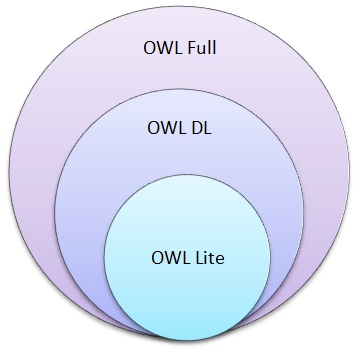
\includegraphics[width=0.3\textwidth]{owl_subset.jpg}
	\caption{Diagram venn profil OWL 1}
	\label{fig:owl_subset}
\end{figure}

OWL-Lite merupakan sub-bagian dari OWL-DL, demikian juga dengan OWL-DL merupakan sub-bagian dari OWL-Full. Gambar \ref{fig:owl_subset} menunjukkan ilustrasi dari \emph{subset} OWL.


\section{OWL 2 Ontologi}
OWL terus dikembangkan seiring dengan semakin pesatnya perkembangan dan kebutuhan akan \emph{knowledge sharing}, oleh karena itu, kelompok kerja ontologi di W3C pada tahun 2012 menetapkan versi baru dari OWL yang disebut dengan OWL 2.0 atau OWL 2.

\begin{figure}[hb]
	\centering
	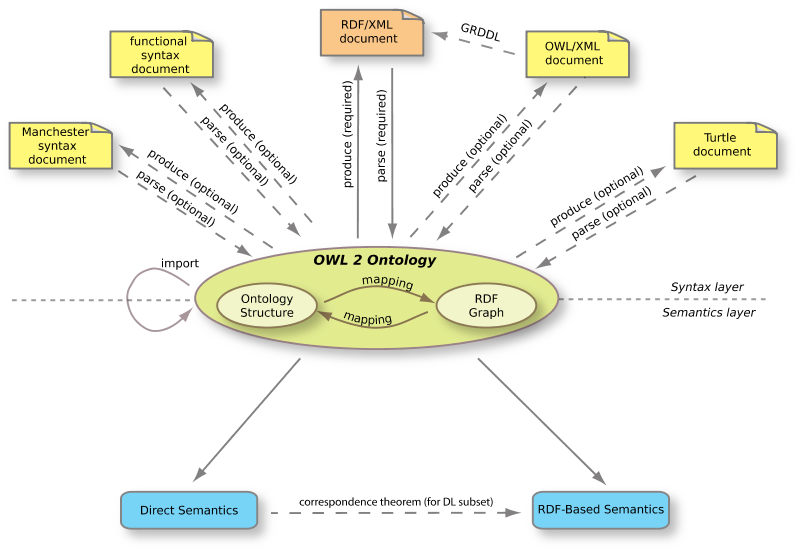
\includegraphics[width=0.8\textwidth]{owl_2_structure}
	\caption{Struktur OWL 2.0}
	\label{fig:owl_2_structure}
\end{figure}

OWL 2 merupakan kelanjutan dari OWL 1.1 dengan beberapa penambahan dan perbaikan fitur. \ref{fig:owl_2_structure} memperlihatkan struktur dasar dari OWL 2.

Bagian atas pada gambar \ref{fig:owl_2_structure} menunjukkan format sintak yang dapat dipergunakan dalam menyusun ontologi dengan menggunakan bahasa OWL 2. Pada OWL 1, format yang dapat digunakan terbatas pada RDF/XML, sedangkan pada OWL 2 seperti yang terlihat dalam gambar \ref{fig:owl_2_structure} terdapat lima buah format yang dapat digunakan. Dari semua format tersebut, W3C hanya mewajibkan format RDF/XML sebagai format standar, sedangkan format lainnya berupa opsional saja.

Masing-masing format sintak memiliki kelebihan dan kekurangan. Format RDF/XML memiliki dukungan yang paling baik, hanya saja kurang intuitif jika dibandingkan dengan Turtle, Functional maupun Manchester, sedangkan Turtle Functional dan Manchester tidak memiliki dukungan \emph{tool} yang baik.

\begin{lstlisting}[language=XML, caption=contoh sintak RDF/XML, xleftmargin=0pt]
	<SubClassOf>
		<Class IRI="Woman"/>
		<Class IRI="Person"/>
	</SubClassOf>
\end{lstlisting}

\begin{lstlisting}[language=XML, caption=contoh sintak functional, xleftmargin=0pt]
	SubClassOf( :Woman :Person )
\end{lstlisting}
	
\begin{lstlisting}[language=XML, caption=contoh manchester syntax, xleftmargin=0pt]
	Class: Woman
		SubClassOf: Person
\end{lstlisting}

\begin{lstlisting}[language=XML, caption=contoh sintak turtle, xleftmargin=0pt]
	:Woman rdfs:subClassOf :Person .
\end{lstlisting}

\subsection{Profil OWL 2}
Seperti yang telah dijelaskan sebelumnya bahwa OWL 1 memiliki tiga sub-bahasa, namun dalam praktiknya ketiga sub-bahasa tersebut ternyata belum cukup untuk memenuhi kebutuhan yang ada. \citet{patel} mengungkapkan beberapa permasalahan dalam \emph{real world application} yang diadapi para pengembang.

\begin{figure}[hb]
	\centering
	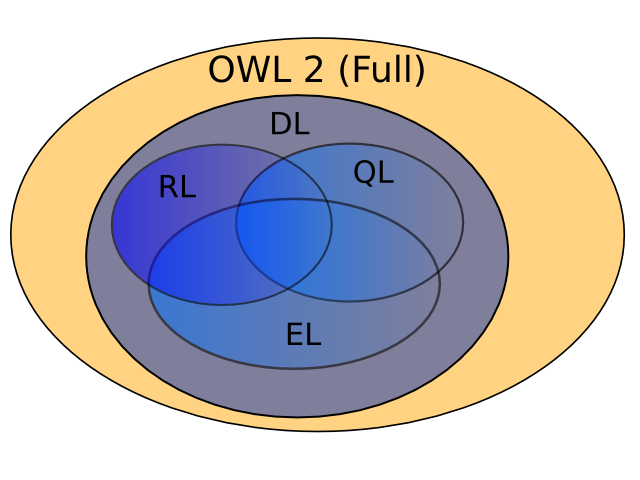
\includegraphics[width=0.4\textwidth]{owl_2_profile}
	\caption{Diagram venn profil OWL 2}
	\label{fig:owl_2_profile}
\end{figure}

Berdasarkan fakta tersebut, maka OWL 2 membagi sub-bahasa kedalam tiga bagian yaitu:
\begin{itemize}
	\item OWL 2 EL
	\item OWL 2 QL
	\item OWL 2 RL
\end{itemize}

Masing-masing profil dibatasi oleh batasan sintaks \emph{(syntactic restriction)}. Perlu diketahui bahwa sub-bahasa OWL 2 ini berdasarkan pada OWL-DL, sehingga semua ekspresi yang diyatakan valid pada OWL 2 EL misalnya, secara otomatis akan valid juga untuk OWL-DL. Gambar \ref{fig:owl_2_profile} menunjukkan diagram venn relasi antar sub-bahasa pada OWL 2.
\section{Ontologi Reasoning}
Proses \emph{reasoning} adalah proses untuk mendapatkan \emph{statement} yang terdapat dalam ontologi namun tidak dinyatakan secara implisit. \citet*{antoniou} menyebutkan beberapa hal yang dapat dihasilkan melalui proses reasoning adalah:
\begin{itemize}
	\item Keanggotaan kelas \emph{(class membership)}. Menentukan apakah sebuah \emph{instance} merupakan anggota dari sebuah kelas. Penentuan keanggotaan ini dilakukan dengan cara memeriksa properti yang dimiliki oleh \emph{instance} tersebut.
	\item Klasifikasi . Apabila terdapat kelas bebek yang merupakan sub-kelas motor dan kelas motor sub-kelas dari kendaraan, maka dapat diperoleh \emph{statement} bahwa kelas bebek adalah sub-kelas dari kendaraan.
	\item Konsistensi dari sebuah ontologi. Untuk menentukan apakah sebuah ontologi konsisten seacara logika dapat pula dilakukan dengan menggunakan proses rasoning. Sebagai contoh, misalnya terdapat dua buah kelas mahasiswa dan dosen yang dinyatakan \emph{disjoint} dan terdapat satu buah \emph{instance} syamsul yang merupakan anggota dari kelas dosen dan mahasiswa, maka ontologi tersebut dikatakan tidak konsisten.
	\item Kesetaraan kelas \emph{equivalence of classes}. Reasoning juga dapat digunakan untuk menentukan ekivalensi kelas, misalnya terdapat kelas kajur yang dinyatakan ekivalen dengan kelas karyawan dan kelas karyawan ekivalen dengan dosen, maka kelas kajur dengan dosen juga ekivalen. 
\end{itemize}
\section{SPARQL \emph{(Sparql Query Language)}}
SPARQL (diucapkan: ``sparkl'') adalah bahasa \emph{query} RDF \emph{(Resource Description Framework)} dan protokol untuk semantik web \citep{liyang_yu}. Secara harfiah, SPARQL adalah bahasa query yang dapat kita gunakan untuk melakukan query terhadap data dalam bentuk RDF dan SPARQL juga menyediakan protokol yang perlu kita ikuti jika ingin melakukan \emph{query} terhadap \emph{remote} RDF \citep{liyang_yu}. Tim Berners-Lee melalui \citet{ducharme} mengungkapkan ``Mencoba menggunakan semantik web tanpa SPARQL sama seperti menggunakan basis data relasional tanpa SQL''.

Rekomendasi W3C \emph{World Wide Web Consortium} mengenai SPARQL terdiri dari tiga bagian, yaitu:

\begin{enumerate}
	\item \emph{SPARQL query language specification} yang membahas mengani inti dari bahasa query SPARQL.
	\item \emph{SPAQRL Query XML Result Format specification} yang membahas mengenai format standar dari kembalian hasil query.
	\item \emph{SPAQRL Protocol for RDF spesification} yang membahas mengenai protokol standar untuk mengakses RDF di lokasi yang berbeda \emph{(remote)}.
\end{enumerate}

Sparql terdiri dari empat buah bentuk query, yaitu (1) SELECT, (2) ASK, (3) DESCRIBE dan (4) CONSTRUCT. Diantara keempat bentuk query tersebut yang paling banyak digunakan adalah SELECT.

\subsection{\emph{SELECT Query}}
SELECT merupakan bentuk query yang paling sering digunakan. Kebanyakan fiturnya juga digunakan pada bentuk query lainnya (ASK, DESCRIBE dan CONSTRUCT). Bentuk dasar \emph{query SELECT} dapat dilihat pada gambar \ref{fig:bentuk_query_select}.
\begin{figure}[b]
	\centering
	\begin{lstlisting}[language=SQL, xleftmargin=15pt, numbers=left]
 	BASE <URI>
 	PREFIX pref: <URI>
 	...
 	SELECT <variabel1> <variabel2>
 	FROM <endpoint>
 	WHERE {
 		...
 	}\end{lstlisting} 
	\caption{Bentuk dasar \emph{query SELECT} \citep{liyang_yu}}
	\label{fig:bentuk_query_select}
\end{figure}

Query \emph{SELECT} diawali dengan mendefinisikan sebuah \emph{base} URI kemudian diikuti dengan \emph{PREFIX}. Jumlah \emph{PREFIX} tidak dibatasi sesuai dengan jumlah URI yang akan dilibatkan dalam melakukan \emph{query}. \emph{PREFIX} dapat pula tidak disertakan karena bersifat opsional. Jika tidak menggunakan \emph{PREFIX} maka \emph{URI} harus diuliskan dengan lengkap.

\begin{figure}[hb]
	\centering
	\begin{lstlisting}[language=SQL, numbers=left]
	base <http://danbri.org/foaf.rdf>
	PREFIX foaf: <http://xmlns.com/foaf/0.1/>

	select * from <http://danbri.org/foaf.rdf>
	where {
		<#danbri> ?propery ?value .
	}\end{lstlisting}
	\caption{Contoh klausa SELECT dalam query SPARQL \citep{liyang_yu}}
	\label{fig:sparql_select_1}
\end{figure}

Klausa \emph{SELECT} digunakan untuk melakukan \emph{binding} terhadap data untuk menentukan data apa saja yang akan dikembalikan sebagai hasil \emph{query}. Klausa \emph{FROM} diletakkan setelah klausa \emph{SELECT}. Klausa ini berfungsi untuk menentukan alamat \emph{endpoint} yang akan dikenakan query.

Bentuk \emph{query SELECT} sederhana ditunjukkan dalam gambar \ref{fig:sparql_select_1}. Baris pertama mendeklarasikan \emph{base} URI, dimana \emph{base} URI merupakan alamat URI umum yang akan dijadikan acuan oleh semua URI yang dituliskan secara relatif di dalam query. Pada gambar \ref{fig:sparql_select_1}, URI relatif ditunjukkan dalam baris ke-6 dimana alamat URI lengkap dari <\#danbri> adalah <http://danbri.org/foaf.org\#danbri>. Perhatikan pada baris ke dua dalam gambar \ref{fig:sparql_select_1} dapat dihilangkan karena bersifat opsional dan tidak pernah diacu dalam \emph{statement where}.

\begin{figure}[hb]
	\centering
	\begin{lstlisting}[language=SQL,numbers=left]
	base <http://danbri.org/foaf.rdf>
	PREFIX foaf: <http://xmlns.com/foaf/0.1/>
	PREFIX dc: <http://purl.org/dc/elements/1.1/>

	select * from <http://danbri.org/foaf.rdf>
	where {
		<#danbri> foaf:knows ?friend .
		?friend foaf:depiction ?picture .
		?picture dc:format ?imageFormat .
	}\end{lstlisting}
	\caption{Klausa \emph{SELECT} dengan banyak \emph{graph-pattern} \citep{liyang_yu}}
	\label{fig:sparql_select_2}
\end{figure}

Contoh lain penggunaan klausa \emph{SELECT} dalam query SPARQL dapat dilihat dalam gambar \ref{fig:sparql_select_2}. \emph{Query} yang ditunjukkan dalam gambar \ref{fig:sparql_select_2} terdiri dari tiga buah \emph{graph pattren} masing-masing ditunjukkan dalam baris 7, 8 dan 9. Berbeda dengan contoh sebelumnya, pada contoh ke dua ini \emph{PREFIX} tidak dapat dihilangkan karena digunakan dalam klausa \emph{where}. 

\begin{figure}[hb]
	\centering
	\begin{lstlisting}[language=SQL,numbers=left]
	base <http://danbri.org/foaf.rdf>
	PREFIX foaf: <http://xmlns.com/foaf/0.1/>
	PREFIX dc: <http://purl.org/dc/elements/1.1/>

	select ?friend,?image from <http://danbri.org/foaf.rdf>
	where {
		<#danbri> foaf:knows ?friend .
		?friend foaf:depiction ?picture .
		?picture dc:format ?imageFormat .
	}\end{lstlisting}
	\caption{Query untuk menampilkan nama dan foto}
	\label{fig:sparql_select_3}
\end{figure}

\emph{Query} pada gambar \ref{fig:sparql_select_2} akan menampilkan semua variabel yang terdapat di dalam klausa \emph{where}. Jika hanya ingin menampilkan variabel tertentu maka tanda ``*'' pada baris ke enam diganti dengan nama variabel yang ingin ditampilkan. Contoh query seperti ini dapat dilihat pada gambar \ref{fig:sparql_select_3}.

\subsection{\emph{Query} Terhadap Multi-Graph}
Contoh \emph{query} yang disajikan dalam gambar \ref{fig:sparql_select_1}, \ref{fig:sparql_select_2} dan \ref{fig:sparql_select_3} hanya melibatkan \emph{graph} tunggal saja, namun demikian SPARQL memungkinkan untuk melakukan \emph{query} terhadap banyak \emph{graph} sekaligus dengan menggunakan metode \emph{named graph}.

\begin{figure}[ht]
	\centering
	\begin{lstlisting}[language=SQL, numbers=left]
		PREFIX foaf: <http://xmlns.com/foaf/0.1/>
		SELECT DISTINCT ?graph_uri ?name ?email
		from named <http://www.liyangyu.com/foaf.rdf>
		from named <http://danbri.org/foaf.rdf>
		where{
			graph ?graph_uri
			{
				?person a foaf:person .
				?person foaf:mbox ?email .
				optional { ?person foaf:name ?name .}
			}
		}
	\end{lstlisting}
	\caption{\emph{Query} terhadap dua buah graph berbeda \citep{liyang_yu}}
	\label{fig:multi_graph_query}
\end{figure}

Implementasi \emph{query} terhadap multi-graph disajikan dalam gambar \ref{fig:multi_graph_query}. Baris ke tiga dan ke empat dalam gambar \ref{fig:multi_graph_query} mendefinisikan dua buah alamat \emph{named graph} yang akan dikenakan query. Baris ke tujuh hingga baris ke sebelas mendefinisikan \emph{graph pattern} yang akan dikenakan terhadap masing-masing \emph{named} graph yang telah di definisikan pada baris ke tiga dan ke empat.
% \section{Ontology Merging}
\section{\textit{Question Answering}}
Semakin banyaknya sumber informasi yang tersedia di internet menyebabkan semakin sulitnya mendapatkan infromasi yang relevan, informasi yang diberikan oleh mesin pencari konvensional saat ini hanya berupa tautan ke laman yang mengandung meta-keyword yang mirip dengan kata kunci yang dimasukkan, pengguna harus membaca terlebih dahulu laman web yang diberikan oleh mesin pencari yang tentu saja akan membutuhkan waktu. Hal ini menjadi tidak efisien terutama apabila yang akan dicari adalah informasi-informasi sederhana seperti informasi cuaca, alamat sebuah instansi dan lain sebagainya. 

Tujuan dari \emph{question answering (QA)} adalah untuk mencari jawaban atas pertanyaan yang diajukan pengguna dalam bentuk terstruktur maupun tidak terstruktur \citep*{moussa_kader}. Pengguna memasukkan pertanyaan dalam bentuk bahasa alami, kemudian sistem akan memproses pertanyaan dan akan menyajikan jawaban yang relevan dalam bentuk teks.

\citet*{ramprasath_hariharan} menyebutkan arsitektur sebuah sistem QA secara umum terdiri dari beberapa modul yaitu:
\begin{enumerate}
	\item Antarmuka pertanyaan \emph{(Query Interface)} \\
		Modul ini berfungsi sebagai penjembatan antara pengguna dengan sistem. Di sinilah pengguna memasukkan kata kunci pencariannya dalam bentuk bahasa alami.
	\item Modul Analisa Pertanyaan \emph{(Query Analyzer)} \\
		Modul ini akan menganalisa subjek, predikat dan objek dari kata kunci yang dimasukkan oleh pengguna.
	\item Modul Klasifikasi Pertanyaan \emph{(Question Classification)} \\
		Bagian ini berfungsi untuk memeriksa tipe dari pertanyaan seperti misalnya \emph{siapa} secara eksplisit menanyakan tentang orang, \emph{kapan}, berhubungan dengan waktu dan lain sebagainya. Klasifikasi ini akan digunakan sebagai pegangan pada tahapan validasi jawaban, apakah jawaban yang diberikan sesui dengan pertanyaan.
	\item Pembentukan Query \emph{(Query Reformulation)} \\
		Modul ini memegang peranan cukup penting, karena bagian ini yang bertanggungjawab atas keabsahan jawaban yang dihasilkan.
	\item Modul Pencari \emph{(Search Engine)} \\ 
		Modul ini digunakan untuk mencari jawaban dari pertayaan yang dihasilkan oleh modul query reformulation. Jawaban akan dicari pada sumber pengetahuan yang telah ditetukan, misalnya laman web ataupun modul basis pengetahuan tertentu seperti ontologi dan lain sebagainya.
	\item Module Ekstraksi \emph{(Answering Extractor)} \\ 
		Kandidat jawaban yang dihasilakan oleh modul search engine kemudian akan dikirimkan ke bagian ini, dimana kandidat jawaban yang umumnya berupa dokumen akan diekstraksi dan selanjutkan akan dikirimkan ke modul penyaring.
	\item Modul Penyaring Jawaban \emph{(Answer Filtering)} \\
		Modul ini akan menyaring kandidat jawaban hasil ekstraksi yang relevan dengan pertanyaan yang diberikan.
	\item Validasi Jawaban \emph{(Answer Validation)} \\ 
		Sebelum jawaban ditampilkan kepada pengguna, terlebih dahulu jawaban akan divalidasi berdasarkan klasifikasi pertanyaan yang telah ditentukan pada modul klasifikasi pertanyaan.
	% \item Ontology Merging \\
	% 	Mesikipun multi-ontologi memiliki kelebihan pada kayanya konsep pengetahuan yang didapat namun demikian oleh karena sangat dimungkinkan masing-masing ontologi yang menjadi sumber informasi ini memiliki struktur yang berbeda, sehingga arsitektur multi-ontologi seperti ini memunculkan tantangan baru yaitu bagaimana menggali informasi dari berbagi ontologi yang tersebar tersebut. Salah satu solusinya adalah dengan menggunakan metode merging.
\end{enumerate}
% \citet*{choi} mendefinisikan ontology-merging sebagai proses pembentukan sebuah ontologi yang mendefinisikan sebuah makna tertentu dari dua buah atau lebih ontologi yang mendefinisikan makna tersebut dengan cara dan bahasa yang berbeda, sehingga diharapkan akan terbentuk sebuah ontologi yang memiliki keseragaman bahasa untuk sebuah konsep tertentu. Ontologi hasil merging memiliki menyimpan informasi dari masing-masing ontologi sumber, namun memiliki keunikan dan bukan merupakan pengganti dari ontologi sumber infromasinya.